% Options for packages loaded elsewhere
\PassOptionsToPackage{unicode}{hyperref}
\PassOptionsToPackage{hyphens}{url}
%
\documentclass[
  10pt,
  a4paper]{article}
\title{Analysis 1B --- Tutorial 5}
\author{Christian Jones: University of Bath}
\date{March 2023}

\usepackage{amsmath,amssymb}
\usepackage{lmodern}
\usepackage{iftex}
\ifPDFTeX
  \usepackage[T1]{fontenc}
  \usepackage[utf8]{inputenc}
  \usepackage{textcomp} % provide euro and other symbols
\else % if luatex or xetex
  \usepackage{unicode-math}
  \defaultfontfeatures{Scale=MatchLowercase}
  \defaultfontfeatures[\rmfamily]{Ligatures=TeX,Scale=1}
\fi
% Use upquote if available, for straight quotes in verbatim environments
\IfFileExists{upquote.sty}{\usepackage{upquote}}{}
\IfFileExists{microtype.sty}{% use microtype if available
  \usepackage[]{microtype}
  \UseMicrotypeSet[protrusion]{basicmath} % disable protrusion for tt fonts
}{}
\makeatletter
\@ifundefined{KOMAClassName}{% if non-KOMA class
  \IfFileExists{parskip.sty}{%
    \usepackage{parskip}
  }{% else
    \setlength{\parindent}{0pt}
    \setlength{\parskip}{6pt plus 2pt minus 1pt}}
}{% if KOMA class
  \KOMAoptions{parskip=half}}
\makeatother
\usepackage{xcolor}
\IfFileExists{xurl.sty}{\usepackage{xurl}}{} % add URL line breaks if available
\IfFileExists{bookmark.sty}{\usepackage{bookmark}}{\usepackage{hyperref}}
\hypersetup{
  pdftitle={Analysis 1B --- Tutorial 5},
  pdfauthor={Christian Jones: University of Bath},
  hidelinks,
  pdfcreator={LaTeX via pandoc}}
\urlstyle{same} % disable monospaced font for URLs
\usepackage[margin=2.5cm]{geometry}
\usepackage{longtable,booktabs,array}
\usepackage{calc} % for calculating minipage widths
% Correct order of tables after \paragraph or \subparagraph
\usepackage{etoolbox}
\makeatletter
\patchcmd\longtable{\par}{\if@noskipsec\mbox{}\fi\par}{}{}
\makeatother
% Allow footnotes in longtable head/foot
\IfFileExists{footnotehyper.sty}{\usepackage{footnotehyper}}{\usepackage{footnote}}
\makesavenoteenv{longtable}
\usepackage{graphicx}
\makeatletter
\def\maxwidth{\ifdim\Gin@nat@width>\linewidth\linewidth\else\Gin@nat@width\fi}
\def\maxheight{\ifdim\Gin@nat@height>\textheight\textheight\else\Gin@nat@height\fi}
\makeatother
% Scale images if necessary, so that they will not overflow the page
% margins by default, and it is still possible to overwrite the defaults
% using explicit options in \includegraphics[width, height, ...]{}
\setkeys{Gin}{width=\maxwidth,height=\maxheight,keepaspectratio}
% Set default figure placement to htbp
\makeatletter
\def\fps@figure{htbp}
\makeatother
\setlength{\emergencystretch}{3em} % prevent overfull lines
\providecommand{\tightlist}{%
  \setlength{\itemsep}{0pt}\setlength{\parskip}{0pt}}
\setcounter{secnumdepth}{5}
\newcommand{\BOO}{BOO}
\usepackage {hyperref}
\hypersetup {colorlinks = true, linkcolor = blue, urlcolor = blue}
\usepackage{float}
\ifLuaTeX
  \usepackage{selnolig}  % disable illegal ligatures
\fi

\usepackage{amsthm}
\theoremstyle{plain}
\newtheorem*{theorem*}{Theorem}\newtheorem{theorem}{Theorem}[section]
\theoremstyle{definition}
\newtheorem*{definition*}{Definition}\newtheorem{definition}{Definition}[section]
\theoremstyle{plain}
\newtheorem*{proposition*}{Proposition}\newtheorem{proposition}[theorem]{Proposition}
\newtheorem*{Definitions*}{Definitions}\newtheorem{Definitions}[definition]{Definitions}
\theoremstyle{plain}
\newtheorem*{lemma*}{Lemma}\newtheorem{lemma}{Lemma}[section]
\theoremstyle{plain}
\newtheorem*{corollary*}{Corollary}\newtheorem{corollary}{Corollary}[section]
\theoremstyle{plain}
\newtheorem*{conjecture*}{Conjecture}\newtheorem{conjecture}{Conjecture}[section]
\theoremstyle{definition}
\newtheorem*{example*}{Example}\newtheorem{example}{Example}[section]
\theoremstyle{definition}
\newtheorem*{exercise*}{Exercise}\newtheorem{exercise}{Exercise}[section]
\newtheorem*{Thought*}{Thought}\newtheorem{Thought}{Thought}[section]
\theoremstyle{remark}
\newtheorem*{remark*}{Remark}
\newtheorem*{solution*}{Solution}
\newtheorem*{Example*}{Example}
\theoremstyle{remark}
\newtheorem*{Proof*}{Proof}
\newtheorem*{Examples*}{Examples}
\let\BeginKnitrBlock\begin \let\EndKnitrBlock\end
\begin{document}
\maketitle

{
\setcounter{tocdepth}{2}
\tableofcontents
}
\newpage
\pagenumbering{arabic}

\hypertarget{introduction}{%
\section*{Introduction}\label{introduction}}
\addcontentsline{toc}{section}{Introduction}

Here is the material to accompany the 5th Analysis 1B Tutorial on the 6th March. Alternative formats can be downloaded by clicking the download icon at the top of the page. Please send any comments or corrections to \href{mailto:caj50@bath.ac.uk}{Christian Jones (caj50)}. To return to the homepage, click \href{http://caj50.github.io/tutoring.html}{here}.

\hypertarget{lecture-recap}{%
\section{Lecture Recap}\label{lecture-recap}}

After what was mainly revision last week, we're moving onto some new stuff again! It turns out there's still a bit we can say about continuity, especially on compact intervals. Finally, we're going to look at differentiation, which gives us a way of describing how fast a function changes.

\hypertarget{inverse-functions}{%
\subsection{Inverse Functions}\label{inverse-functions}}

A particularly useful class of functions we may be interested in are known as invertible. These functions \(f: A \to B\) provide a way of moving between sets \(A\) and \(B\) (and back again) without losing any information about \(A\) and \(B\). Before we talk about them in more detail, it's worth recalling some defintions:
\BeginKnitrBlock{definition}[Injectivity, Surjectivity and Bijectivity]
{\label{def:def1} }Let \(f: A \to B\) be a function.

\begin{itemize}
\tightlist
\item
  If \(\forall x, y \in B\) with \(x \neq y\), \(f(x) = f(y) \implies x = y\), then \(f\) is said to be injective.
\item
  If \(\forall y \in B\), \(\exists x \in A\) such that \(f(x) = y\), then \(f\) is surjective.
\item
  If \(f\) is both injective and surjective, then it is called bijective.
\end{itemize}
\EndKnitrBlock{definition}

In words, bijectivity means that for a function \(f:A \to B\), every element in the codomain \(B\) is mapped to by a unique element in the domain \(A\). These bijective functions are said to be invertible, that is, there exists an inverse function \(f^{-1}: B \to A\) such that \(f^{-1} \circ f\) and \(f \circ f^{-1}\) produce the identity maps on \(A\) and \(B\) respectively.

Now that we have these definitions, we can say something useful about the continuity of inverse functions:

\BeginKnitrBlock{theorem}
{\label{thm:thm1} }Let \(I \subseteq \mathbb{R}\) be a non-empty\footnote{This is so we can talk about surjectivity.} interval, and let \(f: I \to \mathbb{R}\) be continuous on \(I\). Assume that \(f\) is strictly increasing\footnote{In other words, for all \(x,y \in I\) with \(x < y,\) \(f(x) < f(y)\).} (or strictly decreasing) on \(I\). Then:

\begin{itemize}
\tightlist
\item
  \(f(I)\) is an interval,
\item
  \(f : I \to f(I) =: J\) is bijective, and
\item
  \(f^{-1}: J \to I\) is continuous on \(J\).
\end{itemize}
\EndKnitrBlock{theorem}

A (hopefully familiar) example would be useful here:

\BeginKnitrBlock{example}
{\label{exm:unnamed-chunk-2} }Consider the exponential function \(\exp:\mathbb{R} \to \mathbb{R}\) defined by \[f(x)  = \sum_{n = 0}^{\infty} \frac{x^n}{n!} = \mathrm{e}^x.\] Firstly, note that \(\mathbb{R}\) is a non-empty interval. Now, using some results from Semester 1, we know that

\begin{itemize}
\tightlist
\item
  \(\exp\) is continuous and strictly increasing on \(\mathbb{R}\), and
\item
  \(\exp(\mathbb{R}) = (0,\infty)\).
\end{itemize}

Therefore, \(\exp\) satisfies the hypotheses of the above theorem, and so \(\exp: \mathbb{R} \to (0, \infty)\) is a bijection, with continuous inverse. This inverse function is the well-known \emph{natural logarithm} \(\log: (0,\infty) \to \mathbb{R},\) where \(x = \log(y) \iff y = \exp(x).\)
\EndKnitrBlock{example}

This example actually turns out to be really useful if we're dealing with sequences, as we can now prove the following --- hugely general --- result:
\BeginKnitrBlock{proposition}
{\label{prp:prop1} }Let \((a_n)_n\) and \((b_n)_n\) be real sequences such that \(\lim_{n\to\infty}a_n = a\) and \(\lim_{n\to\infty}b_n = b\). If \(a_n^{b_n} \in \mathbb{R}\;\; \forall n \in \mathbb{N}\), and \(a>0\), then \[\lim_{n \to \infty} a_n^{b_n} = \left(\lim_{n\to\infty} a_n\right)^{\lim_{n\to\infty}b_n}.\]
\EndKnitrBlock{proposition}

\textbf{Proof}

\BeginKnitrBlock{proof}
Since \(\lim_{n \to \infty}a_n = a > 0\), then \(\exists N\in\mathbb{N}\) such that \(\forall n \geq N\), \[\lvert a_n - a \rvert < \frac{a}{2} \Longleftrightarrow \frac{a}{2} < a_n < \frac{3a}{2}.\] In particular, \(a_n > 0\) for all \(n \geq N\).

Now, for \(n \geq N\),
\begin{align*}
a_n^{b_n} &= \exp\left(\log\left(a_n^{b_n}\right)\right)\;\;\text{(as $a_n > 0$)},\\
&= \exp\left(b_n\log\left(a_n\right)\right)\;\;\text{(properties of $\log$)}.
\end{align*}
So as \(n \to \infty\) since both \(\exp\) and \(\log\) are continuous,
\begin{align*}
a_n^{b_n} &\to \exp\left(b\log(a)\right)\\
&= \exp\left(\log\left(a^b\right)\right),\\
&= a^b.
\end{align*}
\EndKnitrBlock{proof}

\hypertarget{weierstrass-extremal-theorem}{%
\subsection{Weierstrass Extremal Theorem}\label{weierstrass-extremal-theorem}}

Much like the Intermediate Value Theorem, we can obtain some special continuity results when our functions are defined on compact (i.e.~closed and bounded) intervals. This result is stated below:

\BeginKnitrBlock{theorem}[Weierstrass Extremal Theorem (WET)]
{\label{thm:thm2} }Let \(a,b \in \mathbb{R}\) with \(a<b\), and let\footnote{Recall that \(C^{0}([a,b])\) is the set of continuous functions mapping from the set \([a,b]\).} \(f \in C^{0}([a,b])\). Then:

\begin{enumerate}
\def\labelenumi{\arabic{enumi}.}
\tightlist
\item
  \(f\) is bounded: \[\exists M > 0 \;\;\text{s.t.}\;\; \lvert f(x) \rvert \leq M\;\;\forall x \in [a,b].\]
\item
  \(f\) attains its bounds: \[\exists p,q \in [a,b] \;\; \text{s.t}\;\; \forall x \in [a,b], f(q) \leq f(x) \leq f(p).\]
\end{enumerate}
\EndKnitrBlock{theorem}

This last point states that if \(f \in C^{0}([a,b])\), \[\sup_{x \in [a,b]}f(x) = \max_{x\in[a,b]}f(x)\;\;\text{and}\;\;\inf_{x \in [a,b]}f(x) = \min_{x\in[a,b]}f(x).\] So in fact, what this theorem tells us is that for a function defined on a compact interval, we have some control on its growth, and we know that the function has a maximum and minimum value! This can be seen pictorally in Figure \ref{fig:wet}.

\begin{figure}
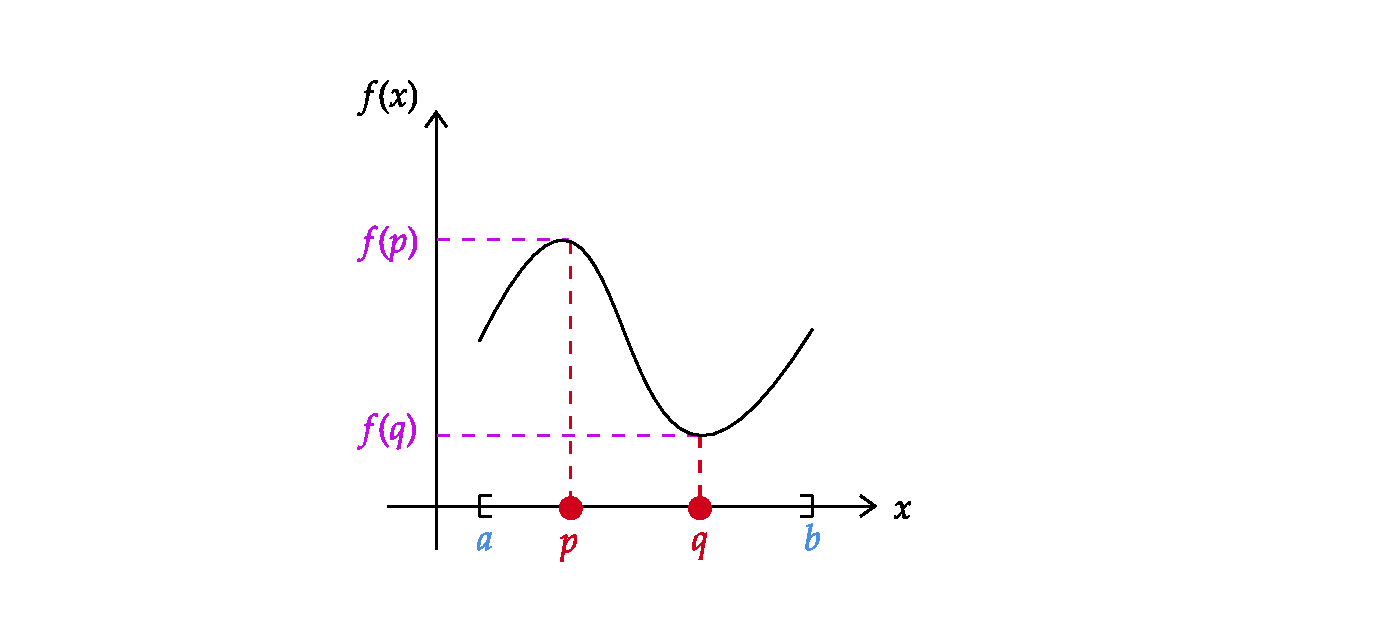
\includegraphics{WET} \caption{This function $f$ is continuous on $[a,b]$, so by the Weierstrass Extremal Theorem, $f$ is bounded on $[a,b]$. Also, we see that there exist points $p$ and $q$ in the domain at which $f$ achieves its maximum and minimum values.}\label{fig:wet}
\end{figure}

\hypertarget{differentiation}{%
\subsection{Differentiation}\label{differentiation}}

While functions are very good at describing physical quantities such as temperature, density or momentum we can usually gain more insight into these variables by studying how fast they change at a given position or time. Mathematically, we study rates of change using derivatives, which again relies on the ideas behind limits!

\BeginKnitrBlock{definition}[Derivative]
{\label{def:def2} }Let \(f: D \to \mathbb{R}\), where \(D \subseteq \mathbb{R}\) is an open set, and let \(c \in D\). Then, if \(\exists L \in \mathbb{R}\) such that \[\lim_{h \to 0}\frac{f(c+h) - f(c)}{h} = L,\] we say that \(f\) is differentiable at \(c\), and call \(L\) the derivative of \(f\) at \(c\).
\EndKnitrBlock{definition}
We can note a few things here:

\begin{itemize}
\tightlist
\item
  Firstly, if this \(L\) exists, we write it as \(f'(c)\) to make it clear that its a derivative.
\item
  We require \(D\) to be open, so that we can actually take limits! If, for example, \(D = [-1,2]\), we could attempt to define the derivative at any point in the interior of \(D\), \(D^{\circ} = (-1,2)\), but we couldn't define the derivative at \(x = -1\) or \(x = 2\).\footnote{There is nothing stopping us; however, defining \emph{left} and \emph{right derivatives} at these points, e.g.~we could search for \[\lim_{x \to -1^{+}}\frac{f(-1+h) - f(-1)}{h}\;\;\text{or}\;\;\lim_{x \to 2^{-}}\frac{f(2+h) - f(2)}{h}.\]}
\item
  Substituting \(x = c+h\) into the definition gives us that equivalently \(f\) is differentiable at \(c\) if there exists \(L\in\mathbb{R}\) such that \[\lim_{x \to c}\frac{f(x) - f(c)}{x - c} = L.\]
\end{itemize}

One quick result we obtain from this definition is the following:
\BeginKnitrBlock{proposition}
{\label{prp:prop2} }If a function \(f:D \to \mathbb{R}\) is differentiable at a point \(c\), then it is continuous at \(c\).
\EndKnitrBlock{proposition}
The contrapositive of this is very useful for ruling functions out: if a function is \textbf{not} continuous, it is not differentiable. As a final remark, or warning, \textbf{continuity does not imply differentiability}! To see this, think of either \(f(x) = \lvert x \rvert\) at \(x = 0\), or look up the \href{https://en.wikipedia.org/wiki/Weierstrass_function}{Weierstrass function}.

\hypertarget{hints}{%
\section{Hints}\label{hints}}

As per usual, here's where you'll find the problem sheet hints!

\begin{enumerate}
\def\labelenumi{\arabic{enumi})}
\tightlist
\item
  This one is largely similar to the one that was covered in tutorials --- you just need to be a bit more careful when verifying the hypothesis of the theorem involving inverse functions. When proving bijectivity, you can use results from tutorial question 1 to help too!
\item
  There are couple of ways to do this, but in each, you need to calculate the limit of the difference quotient, i.e.~\[\lim_{x\to 0 }\frac{f(x) - f(0)}{x - 0}.\] Try using sequences! (Or if you've seen it, try the function version of the pinching theorem).
\item
  Have you learnt any good theorems involving maxima/minima of functions lately?
\end{enumerate}

\end{document}
